\documentclass[cs4size,a4paper,10pt]{ctexart}   

\linespread{1.5}
\usepackage{geometry}%用于设置上下左右页边距
	\geometry{left=2.5cm,right=2.5cm,top=3.2cm,bottom=2.7cm}
\usepackage{xeCJK,amsmath,paralist,enumerate,booktabs,multirow,graphicx,subfig,setspace,listings,lastpage,hyperref}
\usepackage{amsthm, amssymb, bm, color, framed, graphicx, hyperref, mathrsfs}
\usepackage{mathrsfs}  
	\setlength{\parindent}{2em}
	\lstset{language=Matlab}%
\usepackage{fancyhdr}
\usepackage{graphicx}
\usepackage{subfloat}
\usepackage{listings}
\usepackage{xcolor}
\usepackage{float}
\usepackage{paralist}
\usepackage{setspace}
\usepackage{titlesec}
\usepackage{enumitem}
\usepackage{hyperref}
\usepackage{multirow}
\usepackage{threeparttable}



\hypersetup{
	colorlinks=true,
	linkcolor=black
}

\setenumerate{partopsep=0pt,topsep=0pt}
\setitemize{itemsep=0pt,partopsep=0pt,topsep=0pt}

\titlespacing*{\section}{0pt}{3pt}{3pt}
\titlespacing*{\subsection}{0pt}{2pt}{2pt}
\titlespacing*{\subsubsection}{0pt}{1pt}{1pt}
\titlespacing*{\paragraph}{0pt}{0pt}{0pt}

\ctexset{secnumdepth=4,tocdepth=4}
\setlength{\parindent}{0pt}
\setstretch{1.2}


\setCJKmainfont[BoldFont={FZHei-B01},ItalicFont={FZKai-Z03}]{FZShuSong-Z01} 
\setCJKsansfont[BoldFont={FZHei-B01}]{FZKai-Z03} 
\setCJKmonofont[BoldFont={FZHei-B01}]{FZFangSong-Z02}
\setCJKfamilyfont{zhsong}{FZShuSong-Z01} 
\setCJKfamilyfont{zhhei}{FZHei-B01} 
\setCJKfamilyfont{zhkai}[BoldFont={FZHei-B01}]{FZKai-Z03} 
\setCJKfamilyfont{zhfs}[BoldFont={FZHei-B01}]{FZFangSong-Z02} 
\renewcommand*{\songti}{\CJKfamily{zhsong}} 
\renewcommand*{\heiti}{\CJKfamily{zhhei}} 
\renewcommand*{\kaishu}{\CJKfamily{zhkai}} 
\renewcommand*{\fangsong}{\CJKfamily{zhfs}}


\definecolor{mKeyword}{RGB}{0,0,255}          % bule
\definecolor{mString}{RGB}{160,32,240}        % purple
\definecolor{mComment}{RGB}{34,139,34}        % green
\definecolor{mNumber}{RGB}{128,128,128} 

\lstdefinestyle {njulisting} {
	basewidth = 0.5 em,
	lineskip = 3 pt,
	basicstyle = \small\ttfamily,
	% keywordstyle = \bfseries,
	commentstyle = \itshape\color{gray}, 
	basicstyle=\small\ttfamily,
	keywordstyle={\color{mKeyword}},     % sets color for keywords
	stringstyle={\color{mString}},       % sets color for strings
	commentstyle={\color{mComment}},     % sets color for comments
	numberstyle=\tiny\color{mNumber},
	numbers = left,
	captionpos = t,
	breaklines = true,
	xleftmargin = 2 em,
	xrightmargin = 2 em,
	frame=tlrb,
	tabsize=4
}

\lstset{
style = njulisting, % 调用上述样式 
flexiblecolumns % 允许调整字符宽度
}


%================= 基本格式预置 ===========================
\usepackage{fancyhdr}
\pagestyle{fancy}
\lhead{\textsc{Computer Networking}}
\rhead{第二章\ 物理层}
\cfoot{\thepage}
\renewcommand{\headrulewidth}{0.4pt}
\renewcommand{\theenumi}{(\arabic{enumi})}
\CTEXsetup[format={\bfseries\zihao{-3}}]{section}
\CTEXsetup[format={\bfseries\zihao{4}}]{subsection}
\CTEXsetup[format={\bfseries\zihao{-4}}]{subsubsection}


\renewcommand{\contentsname}{目录}  
\begin{document}

	\begin{center}
		{\huge\textbf{第二章\ 物理层}}
	\end{center}
	%---------目录---------% 
	\pagenumbering{Roman}
	\tableofcontents
	\clearpage

 	%---------正文---------% 
	\pagenumbering{arabic}
	\setcounter{page}{1}
	\setlength{\parskip}{0.65em}
	
	\section{物理层的基本概念}

	\begin{itemize}
		\item 物理层考虑的是怎样才能在连接各种计算机的传输媒体上传输数据比特流,而不是指具体的传输媒体
		\item 用于物理层的协议也常称为物理层规程(procedure)
		\item 可以将物理层的主要任务描述为确定与传输媒体的接口有关的一些特性,即:
		\begin{itemize}
			\item 机械特性:指明接口所用接线器的形状和尺寸、引脚数目和排列、固定和锁定装置等。平时常见的各种规格的接插件都有严格的标准化的规定
			\item 电气特性:指明在接口电缆的各条线上出现的电压的范围
			\item 功能特性:指明某条线上出现的某一电平的电压的意义
			\item 过程特性:指明对于不同功能的各种可能事件的出现顺序
		\end{itemize}
	\end{itemize}


	\section{数据通信的基础知识}

	\subsection{数据通信系统的模型}

	一个数据通信系统可划分为三大部分,即源系统(或发送端、发送方)、传输系统(或传输网络)和目的系统(或接收端、接收方)
	\begin{itemize}
		\item 源系统一般包括以下两个部分:
		\begin{itemize}
			\item 源点(source):源点设备产生要传输的数据,又称为源站或信源
			\item 发送器:通常源点生成的数字比特流要通过发送器编码后才能够在传输系统中进行传输。典型的发送器就是调制器。现在很多计算机使用内置的调制解调器(包含调制器和解调器)
		\end{itemize}
		\item 目的系统一般也包括以下两个部分:
		\begin{itemize}
			\item 接收器:接收传输系统传送过来的信号,并把它转换为能够被目的设备处理的信息。典型的接收器就是解调器,它把来自传输线路上的模拟信号进行解调,提取出 在发送端置入的消息,还原出发送端产生的数字比特流
			\item 终点(destination):终点设备从接收器获取传送来的数字比特流,然后把信息输出,又称为目的站或信宿
		\end{itemize}
		\item 在源系统和目的系统之间的传输系统可以是简单的传输线,也可以是连接在源系统和目的系统之间的复杂网络系统
	\end{itemize}

	\begin{figure}[H]
		\centering
		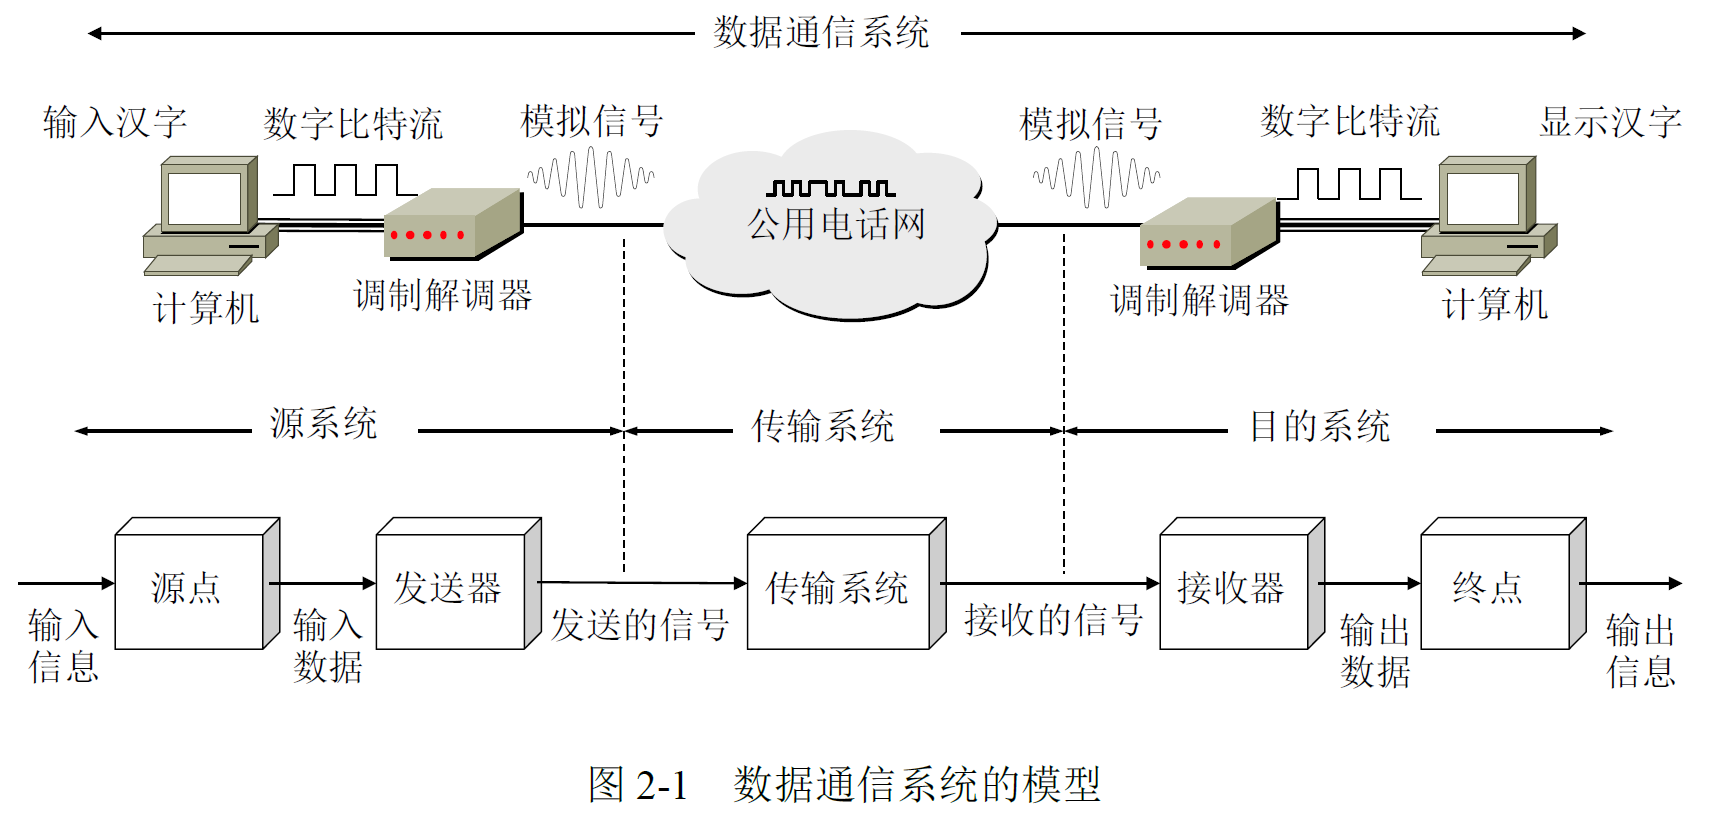
\includegraphics[width=0.9\textwidth]{img/2.1}
	\end{figure}

	\subsection{有关信道的几个基本概念}
	\begin{itemize}
		\item 信道一般用来表示向某一个方向传送信息的媒体。因此,一条通信电路往往包含一条发送信道和一条接收信道
		\item 从通信的双方信息交互的方式来看,可以有以下三种基本方式:
		\begin{itemize}
			\item 单向通信,又称为单工通信,即只能有一个方向的通信而没有反方向的交互
			\item 双向交替通信,又称为半双工通信,即通信的双方都可以发送信息,但不能双方同时发送(接收)
			\item 双向同时通信,又称为全双工通信,即通信的双方可以同时发送和接收信息
		\end{itemize}
		\item 来自信源的信号常称为基带信号(即基本频带信号)
		\item 由于基带信号往往包含有较多的低频成分,甚至有直流成分,而许多信道并不能传输这种低频分量或直流分量,所以必须对基带信号进行调制(modulation)
		\begin{itemize}
			\item 基带调制:仅仅对基带信号的波形进行变换,使它能够与信道特性相适应。变换后的信号仍然是基带信号。由于这种基带调制是把数字信号转换为另一种形式的数字信号,因此大家更愿意把这种过程称为编码(coding)
			\item 带通调制:使用载波(carrier)进行调制,把基带信号的频率范围搬移到较高的频段,并转换为模拟信号,这样就能够更好地在模拟信道中传输
		\end{itemize}
	\end{itemize}

	\subsubsection{常用编码方式}

	\begin{figure}[H]
		\centering
		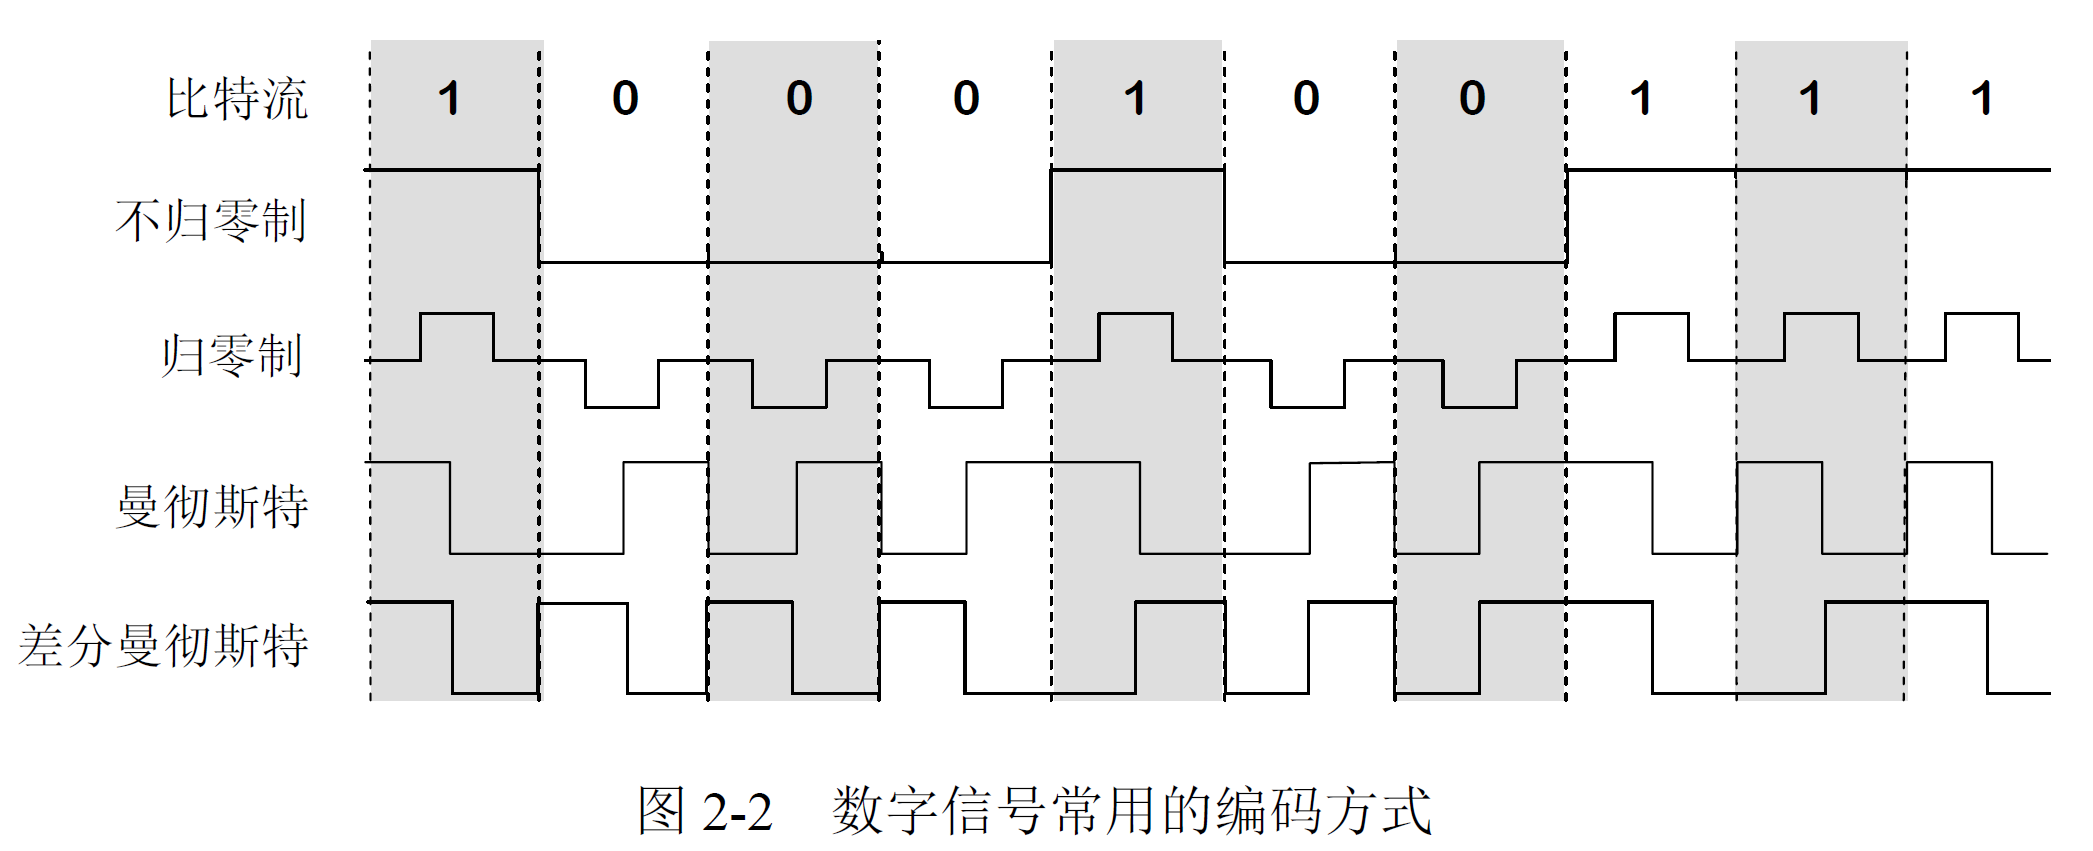
\includegraphics[width=0.6\textwidth]{img/2.2}
	\end{figure}

	\begin{itemize}
		\item 不归零制:正电平代表 1,负电平代表 0
		\item 归零制:正脉冲代表 1,负脉冲代表 0
		\item 曼彻斯特编码:位周期中心的向上跳变代表0,位周期中心的向下跳变代表1;也可反过来定义
		\item 差分曼彻斯特编码:在每一位的中心处始终都有跳变。位开始边界有跳变代表0,而位开始边界没有跳变代表1
	\end{itemize}

	\subsubsection{基本的带通调制方法}

	\begin{figure}[H]
		\centering
		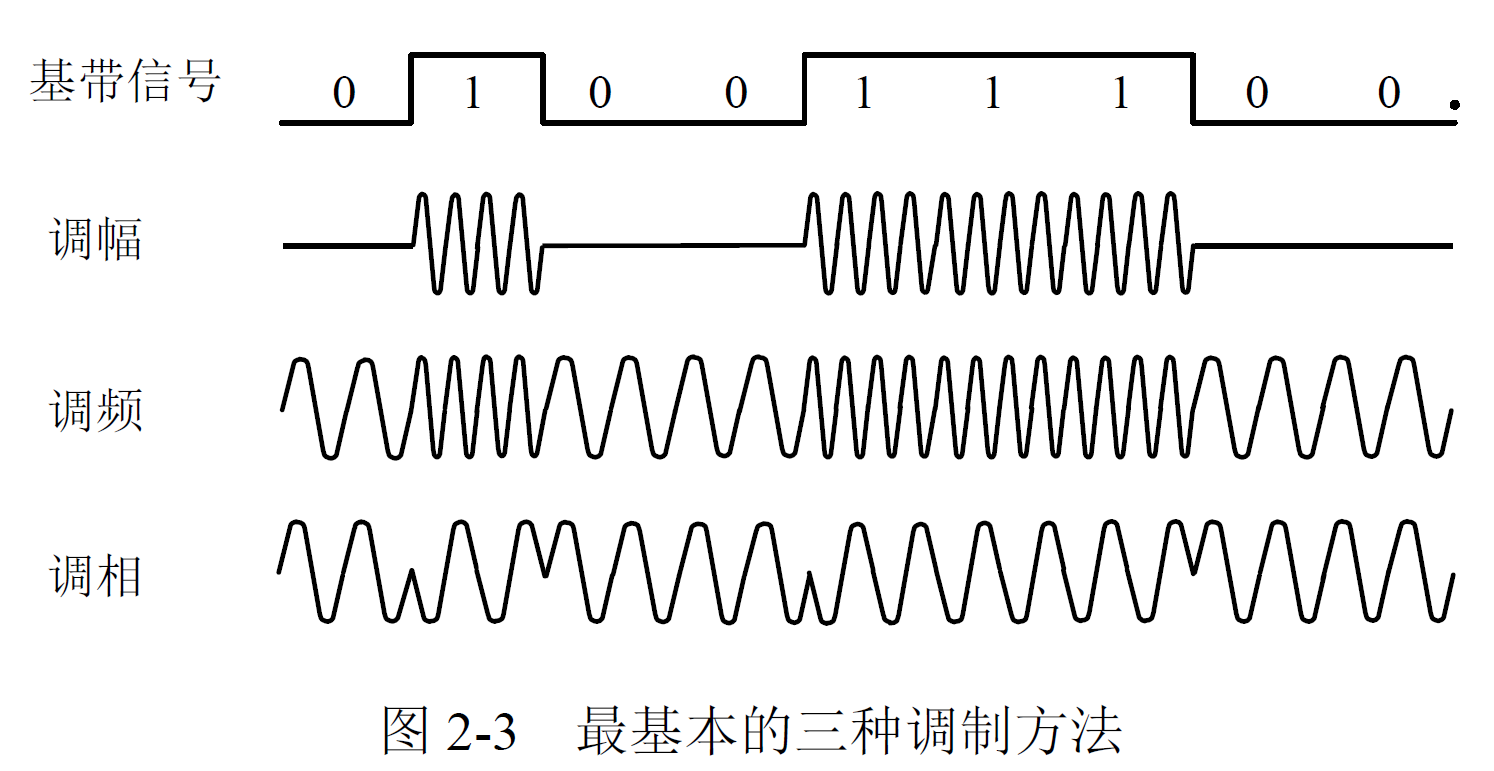
\includegraphics[width=0.45\textwidth]{img/2.3}
	\end{figure}
	为了达到更高的信息传输速率,必须采用技术上更为复杂的多元制的振幅相位混合调制方法。例如,正交振幅调制 QAM (Quadrature Amplitude Modulation)

	\subsection{信道的极限容量}
	\begin{figure}[H]
		\centering
		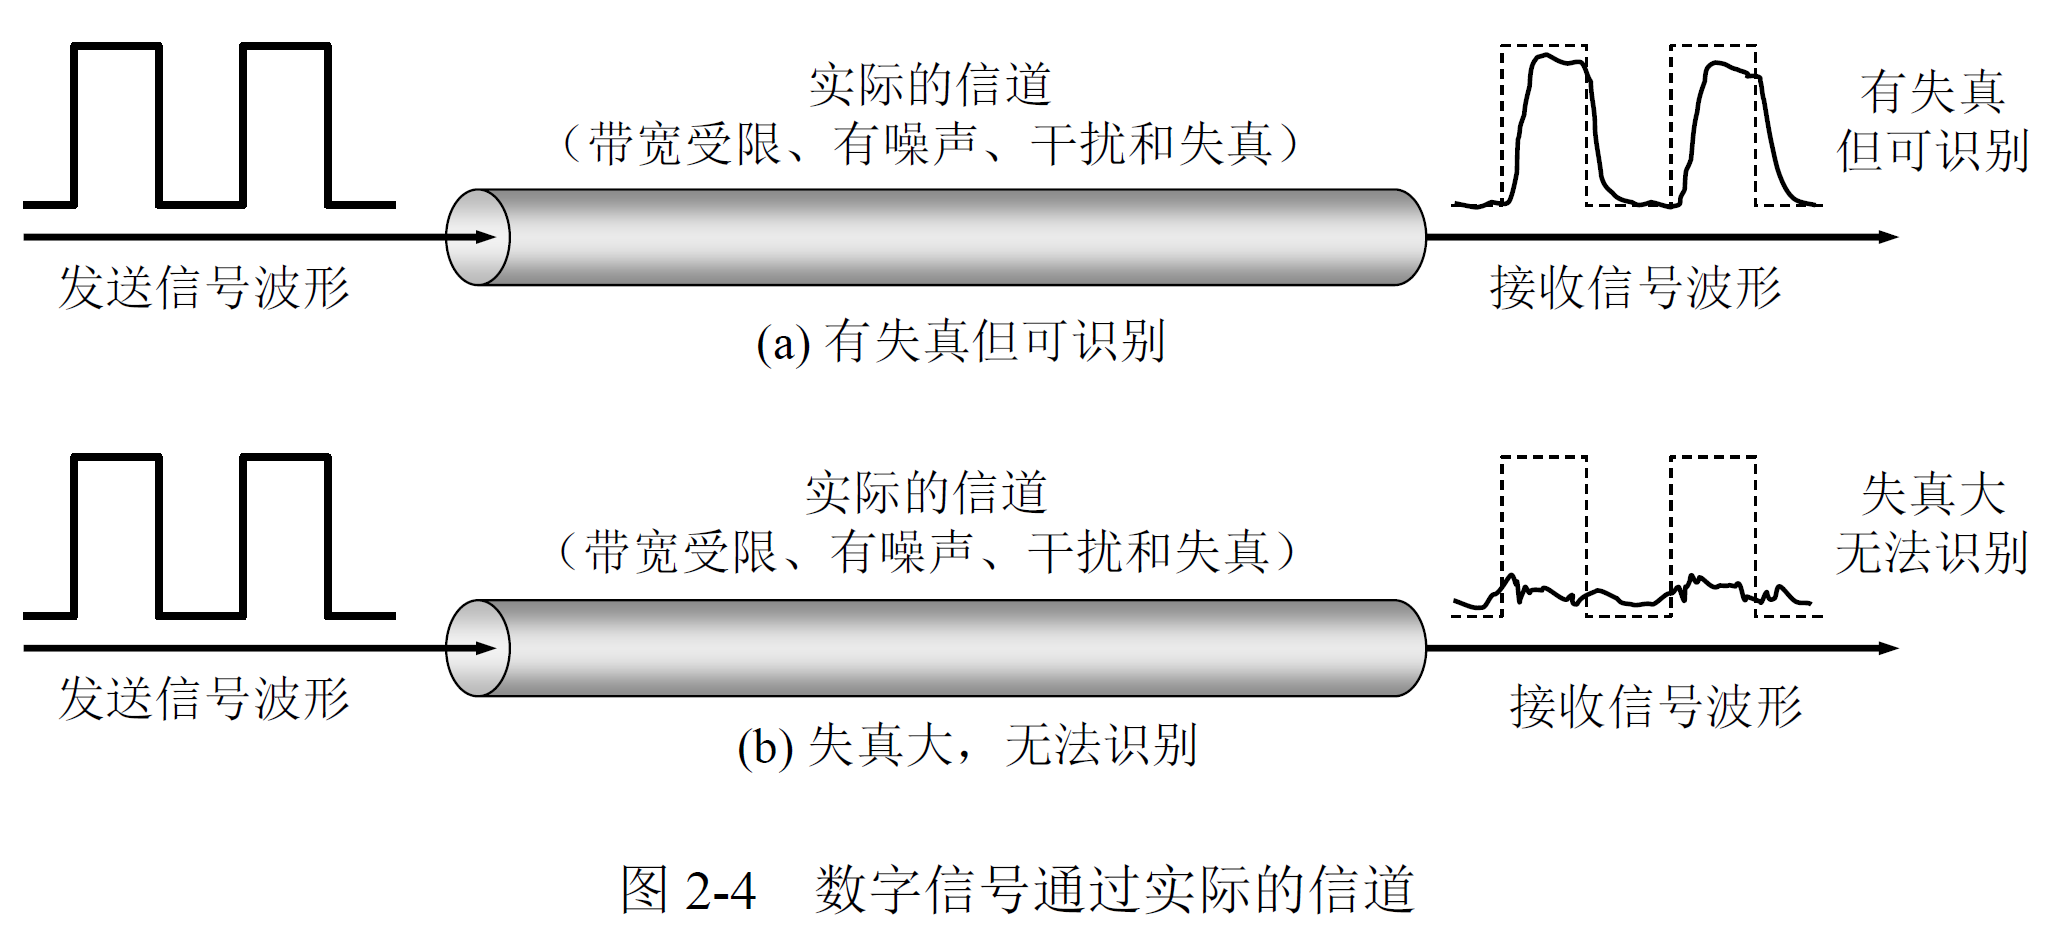
\includegraphics[width=0.7\textwidth]{img/2.4}
	\end{figure}
	从概念上讲,限制码元在信道上的传输速率的因素有:
	\begin{itemize}
		\item 信道能够通过的频率范围
		\item 信噪比
	\end{itemize}

	\subsubsection{奈氏准则}
	\begin{itemize}
		\item 在假定的理想条件下,为了避免码间串扰,码元传输速率是有上限的
		\item 用$W$表示信号带宽(单位为Hz), $\mathrm{Baud}$为波特,即码元/秒,则有:
		$$
		\begin{aligned}
		& \mbox{理想低通信道的最高码元传输速率}=2W\ \mathrm{Baud}=2W\ \mbox{码元/秒} \\
		& \mbox{理想带通信道的最高码元传输速率}=W\ \mathrm{Baud}=W\ \mbox{码元/秒}
		\end{aligned}
		$$
		\item 码元传输速率又称为波特率、调制频率、波形频率或符号频率。它与比特率有一定关系:
		\begin{itemize}
			\item 当1个码元只携带1比特的信息量时,则波特率(码元/秒)与比特率(比特/秒)在数值上是相等的
			\item 当1个码元携带$n$比特的信息量时,则波特率转换成比特率时,数值要乘以$n$
		\end{itemize}
		\item 要提高信息传输速率(比特率),就必须设法使每一个码元能携带更多个比特的信息量。这需要采用多元制
		\item 实际的信道所能传输的最高码元速率,要明显低于奈氏准则给出的上限数值
	\end{itemize}

	\subsubsection{香农公式}

	\begin{itemize}
		\item 香农公式描述的是带宽受限且有高斯白噪声干扰的信道的极限信息传输速率
		\item 用$W$​表示信道带宽(单位Hz),$S$​表示信道内所传信号的平均功率,$N$​表示信道内的高斯噪声功率,$S/N$​​表示信噪比,使用分贝(dB)作为度量单位,且有
		$$
		\mbox{信噪比}\ \mathrm{(dB)}=10\times \log_{10} \frac{S}{N}\ \mathrm{(dB)}
		$$
		则信道的极限信息传输速率$c$​表示为(单位b/s)
		$$c=W\times \log_2\left(1+\frac{S}{N}\right)$$
	\end{itemize}


	\section{物理层下面的传输媒体}

	\begin{itemize}
		\item 传输媒体是数据传输系统中在发送器和接收器之间的物理通路,也称为传输介质或传输媒介
		\item 传输媒体可分为两大类:导引型传输媒体和非导引型传输媒体
		\begin{itemize}
			\item 在导引型传输媒体中,电磁波被导引沿着固体媒体(铜线或光纤)传播
			\item 非导引型传输媒体就是指自由空间,在非导引型传输媒体中电磁波的传输常称为无线传输
		\end{itemize}
	\end{itemize}

	\begin{figure}[H]
		\centering
		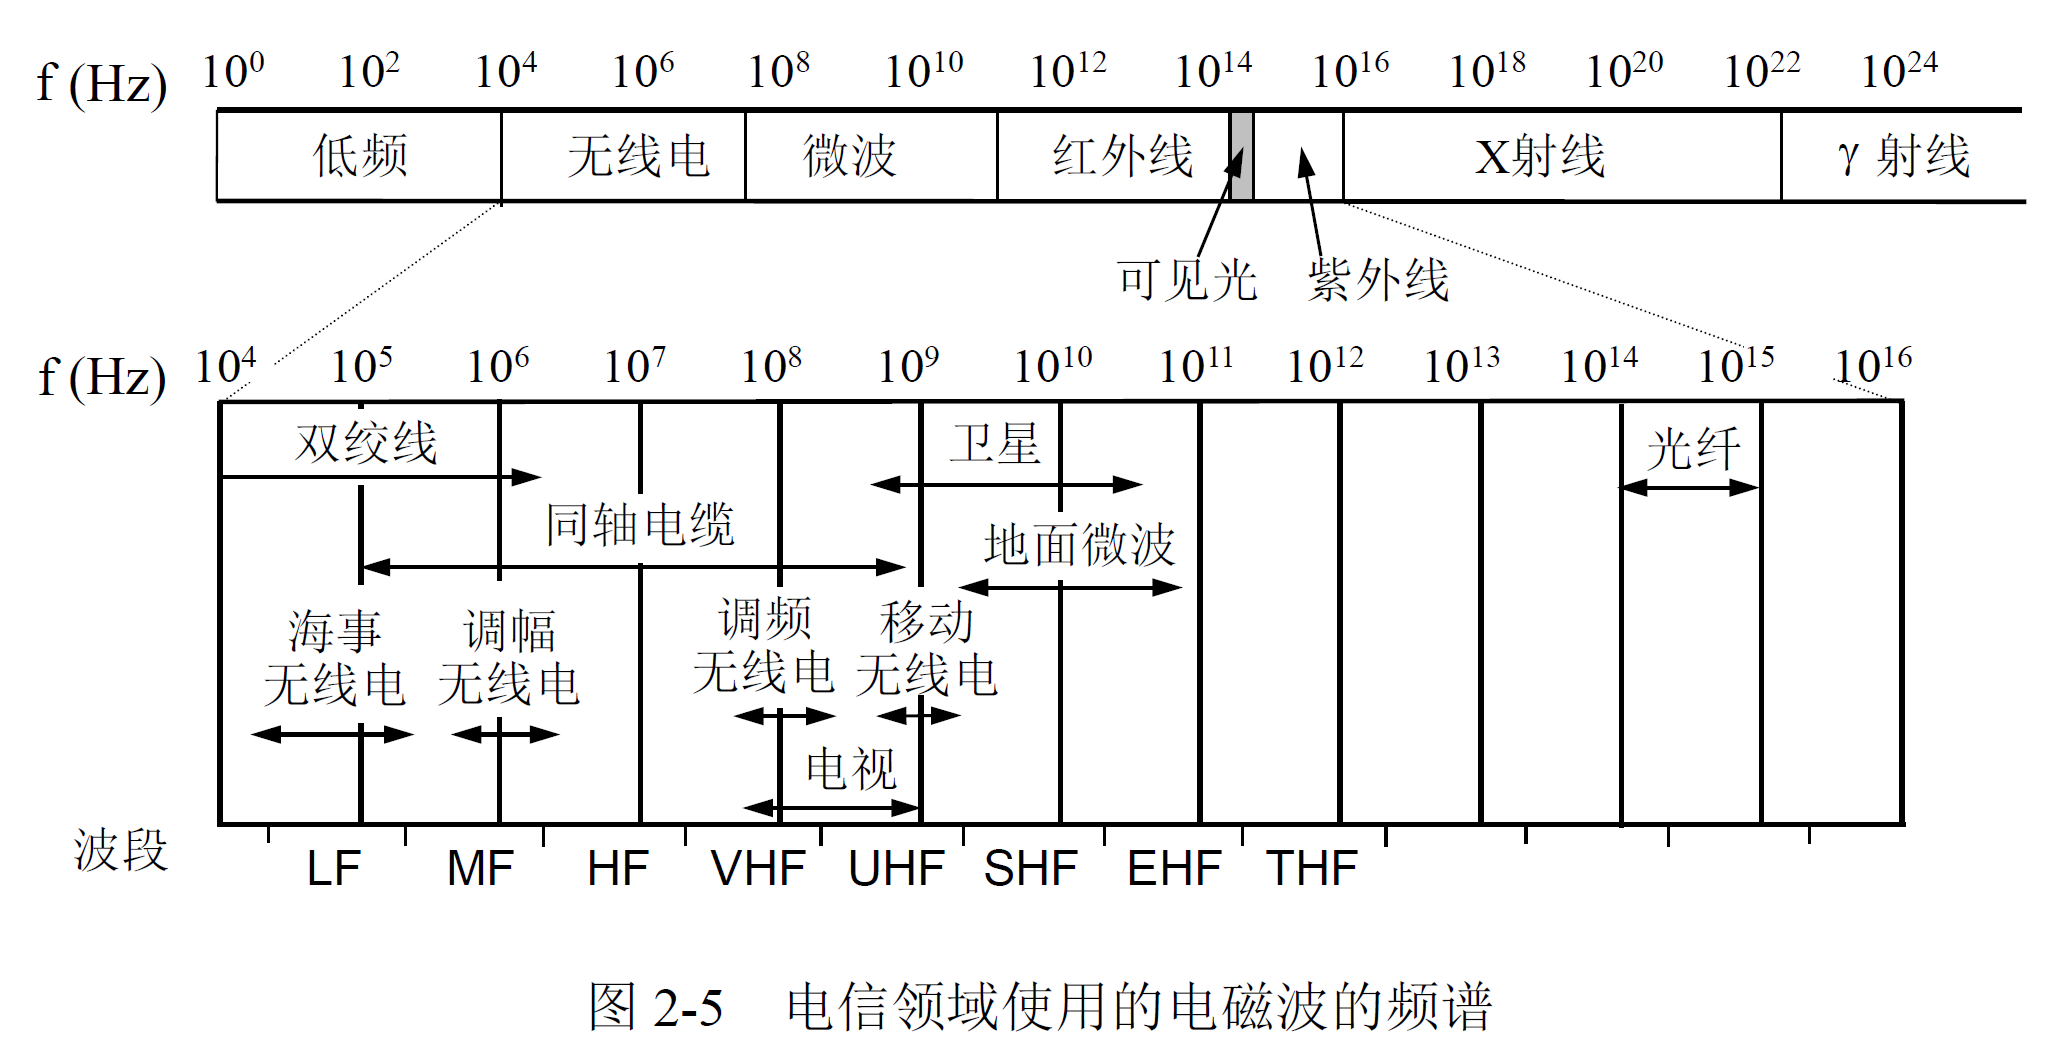
\includegraphics[width=0.8\textwidth]{img/2.5}
	\end{figure}

	\subsection{导引型传输媒体}

	\subsubsection{双绞线}
	\begin{itemize}
		\item 把两根互相绝缘的铜导线并排放在一起,然后用规则的方法绞合起来就构成了双绞线
		\item 绞合可减少相邻导线的电磁干扰,也可抵御部分来自外界的电磁波干扰
		\item 为了提高双绞线抗电磁干扰的能力,可以在双绞线的外面再加上一层用金属丝编织成的屏蔽层。这就是屏蔽双绞线,简称为 STP
	\end{itemize}

	\begin{figure}[H]
		\centering
		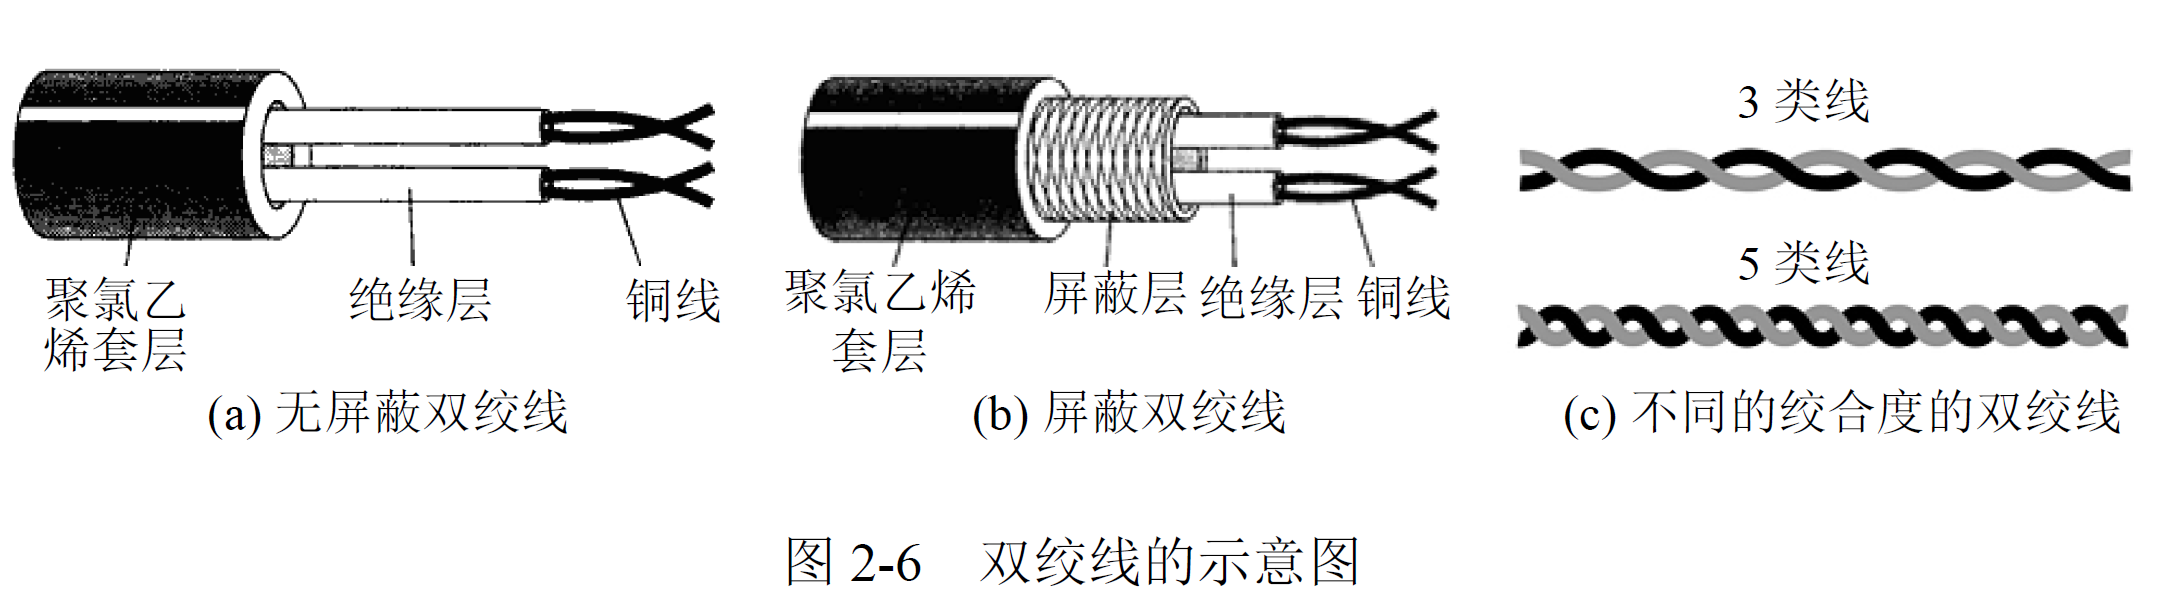
\includegraphics[width=0.9\textwidth]{img/2.6}
	\end{figure}

	\subsubsection{同轴电缆}
	同轴电缆由内导体铜质芯线(单股实心线或多股绞合线)、绝缘层、网状编织的外导体屏蔽层(也可以是单股的)以及保护塑料外层所组成

	由于外导体屏蔽层的作用,同轴电缆具有很好的抗干扰特性,被广泛用于传输较高速率的数据

	\begin{figure}[H]
		\centering
		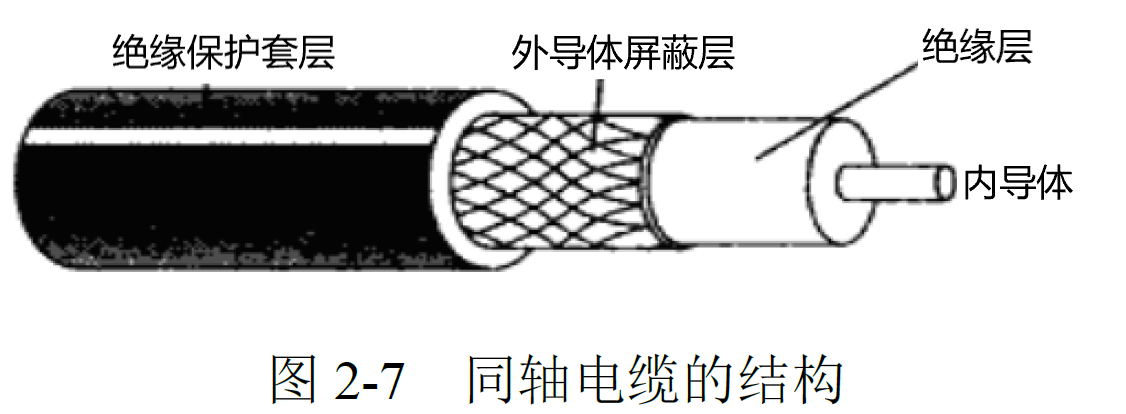
\includegraphics[width=0.35\textwidth]{img/2.7}
	\end{figure}

	\subsubsection{光纤}
	\begin{itemize}
		\item 光纤是光纤通信的传输媒体。在发送端有光源,可以采用发光二极管或半导体激光器,它们在电脉冲的作用下能产生出光脉冲。在接收端利用光电二极管做成光检测器,在检测到光脉冲时可还原出电脉冲
		\item 光纤通常由非常透明的石英玻璃拉成细丝,主要由纤芯和包层构成双层通信圆柱体
	\end{itemize}

	\begin{figure}[H]
		\centering
		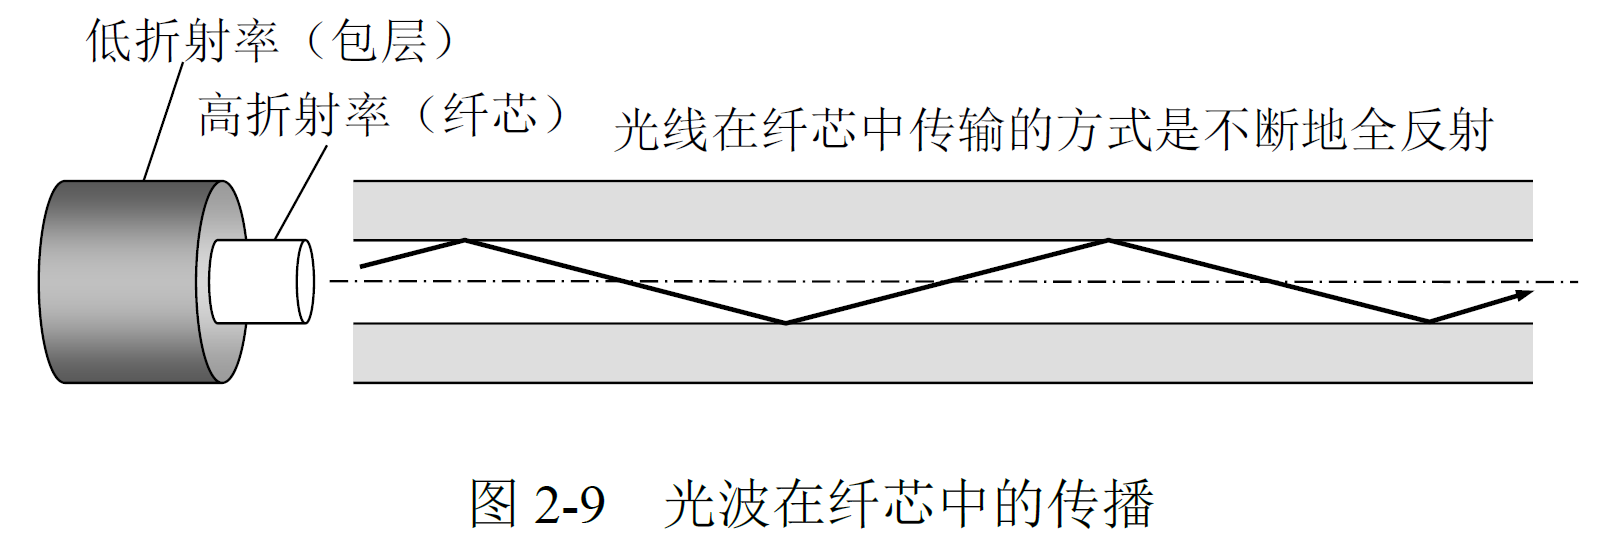
\includegraphics[width=0.55\textwidth]{img/2.9}
	\end{figure}

	\begin{itemize}
		\item 可以存在多条不同角度入射的光线在一条光纤中传输,这种光纤就称为多模光纤。光脉冲在多模光纤中传输时会逐渐展宽,造成失真。因此多模光纤只适合于近距离传输
		\item 若光纤的直径减小到只有一个光的波长,则光纤就像一根波导那样,它可使光线一直向前传播,而不会产生多次反射,这样的光纤称为单模光纤
	\end{itemize}

	\begin{figure}[H]
		\centering
		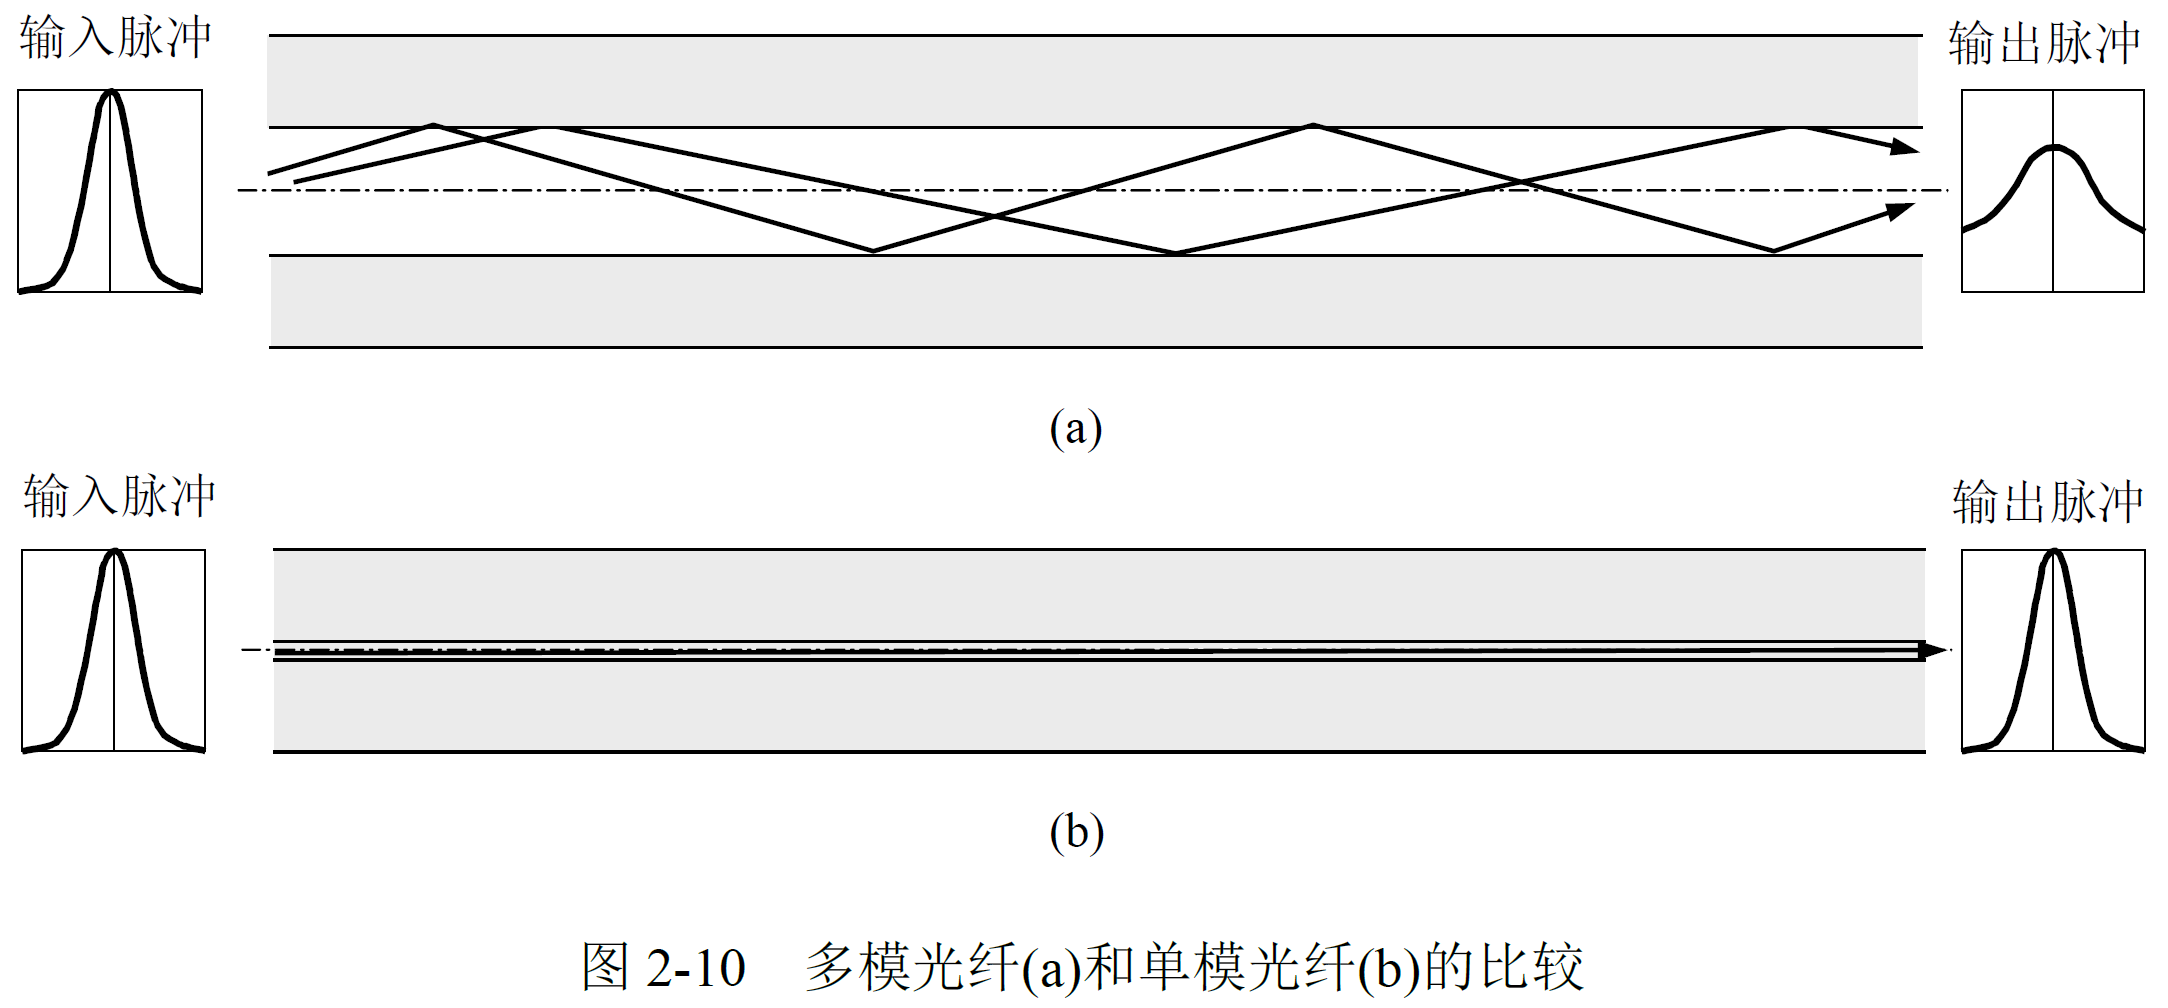
\includegraphics[width=0.55\textwidth]{img/2.10}
	\end{figure}

	\begin{itemize}
		\item 由于光纤非常细,因此必须将光纤做成很结实的光缆
	\end{itemize}

	\begin{figure}[H]
		\centering
		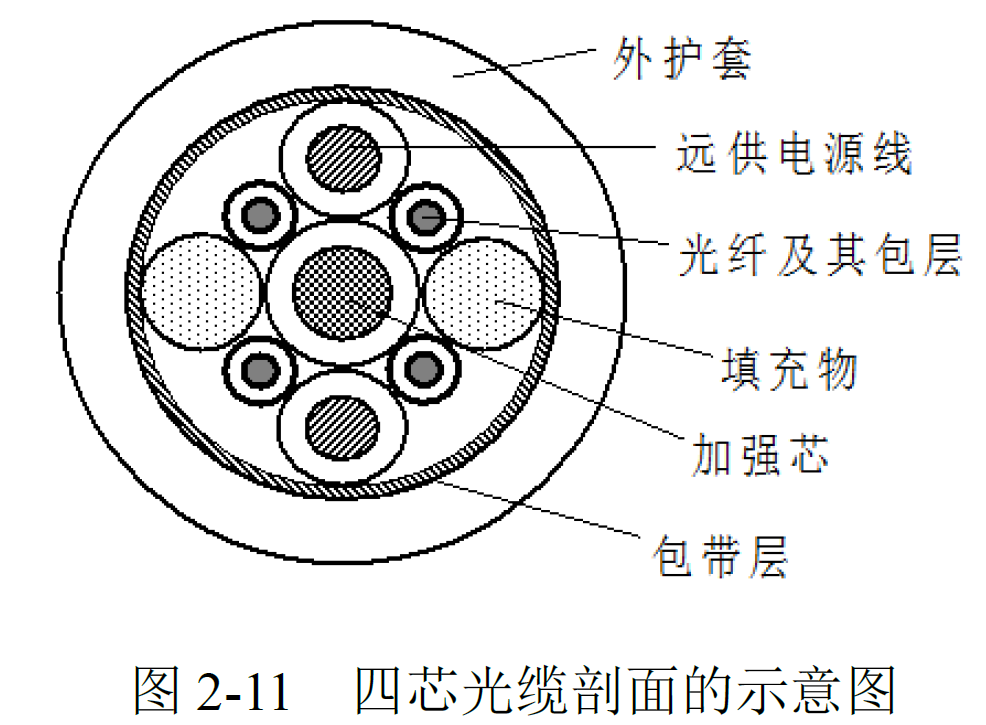
\includegraphics[width=0.3\textwidth]{img/2.11}
	\end{figure}

	\begin{itemize}
		\item 光纤的优点
		\begin{itemize}
			\item 传输损耗小,中继距离长,对远距离传输特别经济
			\item 抗雷电和电磁干扰性能好,这在有大电流脉冲干扰的环境下尤为重要
			\item 无串音干扰,保密性好,也不易被窃听或截取数据
			\item 体积小,重量轻
		\end{itemize}
		\item 光纤的缺点
		\begin{itemize}
			\item 割接需要专用设备
			\item 光电接口价格较贵
		\end{itemize}
	\end{itemize}

	\subsection{非导引型传输媒体}
	短波通信主要是靠电离层的反射。但电离层的不稳定所产生的衰落现象和电离层反射所产生的多径效应,使得短波信道的通信质量较差,因此,当必须使用短波无线电台传送数据时,一般都是低速传输

	无线电微波通信主要使用 2$\sim$40 GHz 的频率范围。微波在空间主要是直线传播。由于微波会穿透电离层而进入宇宙空间,因此它不像短波那样可以经电离层反射传播到地面上很远的地方。传统的微波通信主要有两种方式,即地面微波接力通信和卫星通信

	卫星通信的最大特点是通信距离远,且通信费用与通信距离无关,但具有较大的传播时延

	\section{信道复用技术}

	\subsection{频分复用、时分复用和统计时分复用}

	\begin{figure}[H]
		\centering
		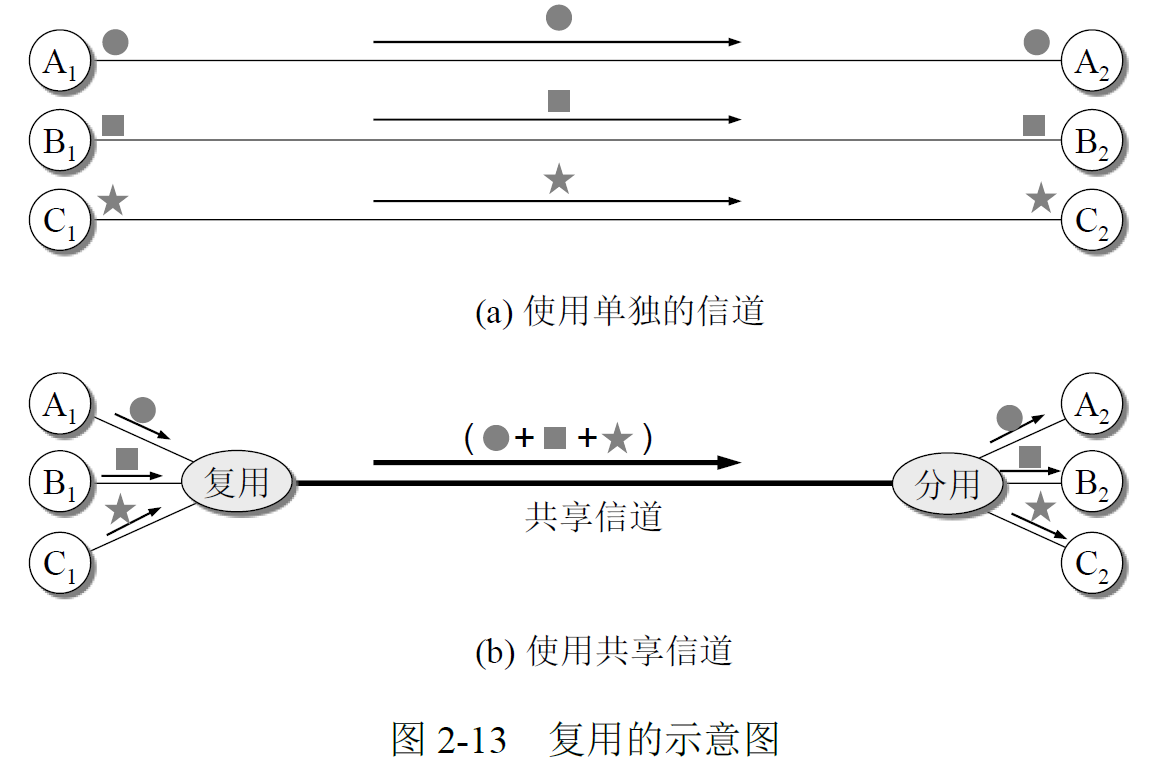
\includegraphics[width=0.6\textwidth]{img/2.13}
	\end{figure}

	最基本的复用就是频分复用 FDM(Frequency Division Multiplexing)和时分复用 TDM(Time Division Multiplexing)
	\begin{itemize}
		\item 频分复用:用户在分配到一定的频带后,在通信过程中自始至终都占用这个频带。频分复用的所有用户在同样的时间占用不同的带宽资源(请注意,这里的“带宽”是频率带宽而不是数据的发送速率)
		\item 时分复用:将时间划分为一段段等长的时分复用帧(TDM 帧)。每一个时分复用的用户在每一个 TDM 帧中占用固定序号的时隙。时分复用的所有用户是在不同的时间占用同样的频带宽度
	\end{itemize}

	\begin{figure}[H]
		\centering
		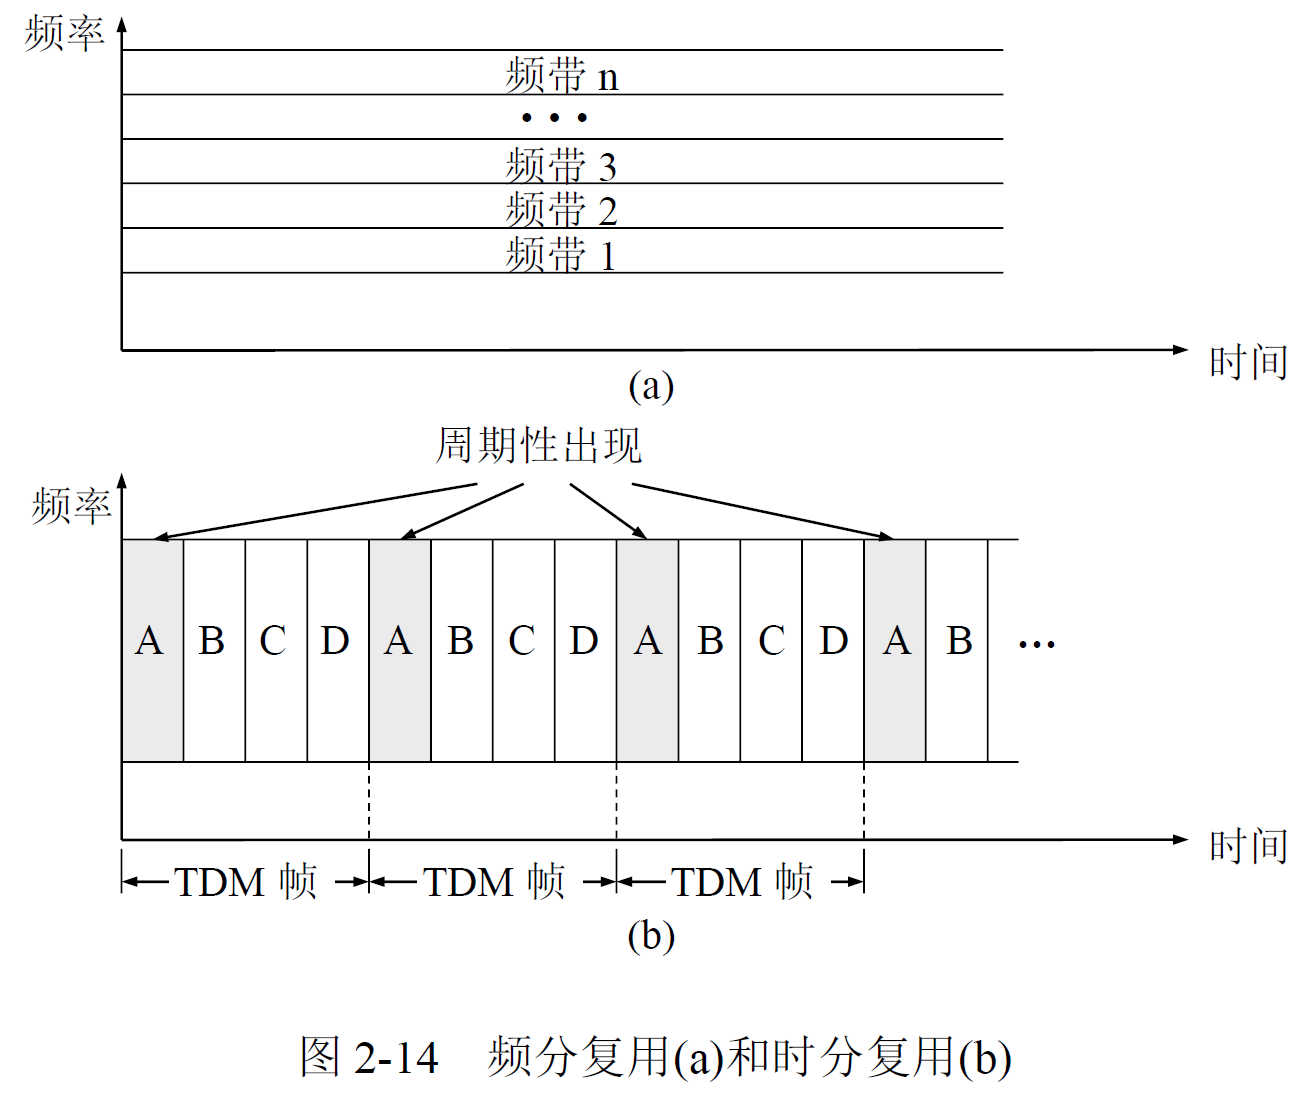
\includegraphics[width=0.6\textwidth]{img/2.14}
	\end{figure}

	\begin{itemize}
		\item 统计时分复用STDM (Statistic TDM)是一种改进的时分复用,它能明显地提高信道的利用率。集中器(concentrator)常使用这种统计时分复用
	\end{itemize}

	
	\begin{figure}[H]
		\centering
		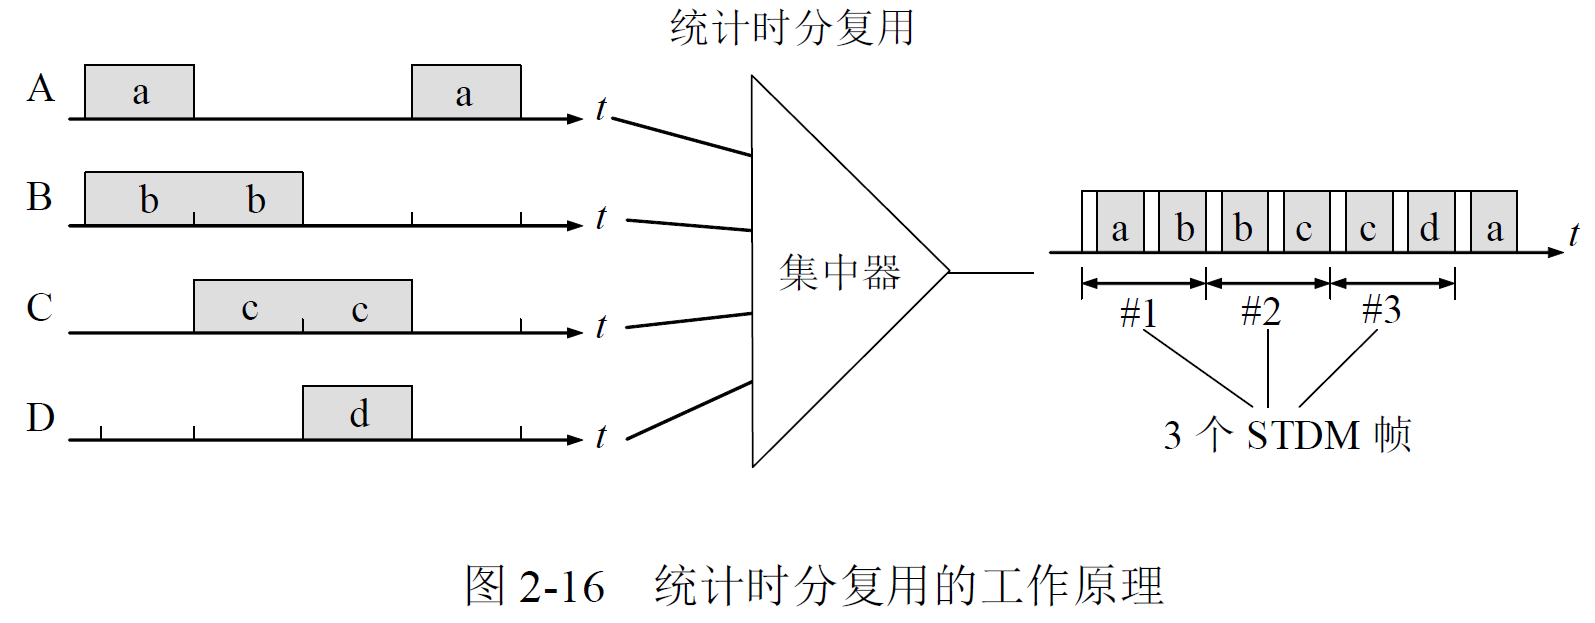
\includegraphics[width=0.75\textwidth]{img/2.16}
	\end{figure}

	\subsection{波分复用}
	波分复用 WDM(Wavelength Division Multiplexing)就是光的频分复用

	由于光信号一段距离后就会衰减,因此对衰减了的光信号必须进行放大才能继续传输。采用掺铒光纤放大器 EDFA  能使两个放大器之间的光缆线路长度达到 120 km

	\begin{figure}[H]
		\centering
		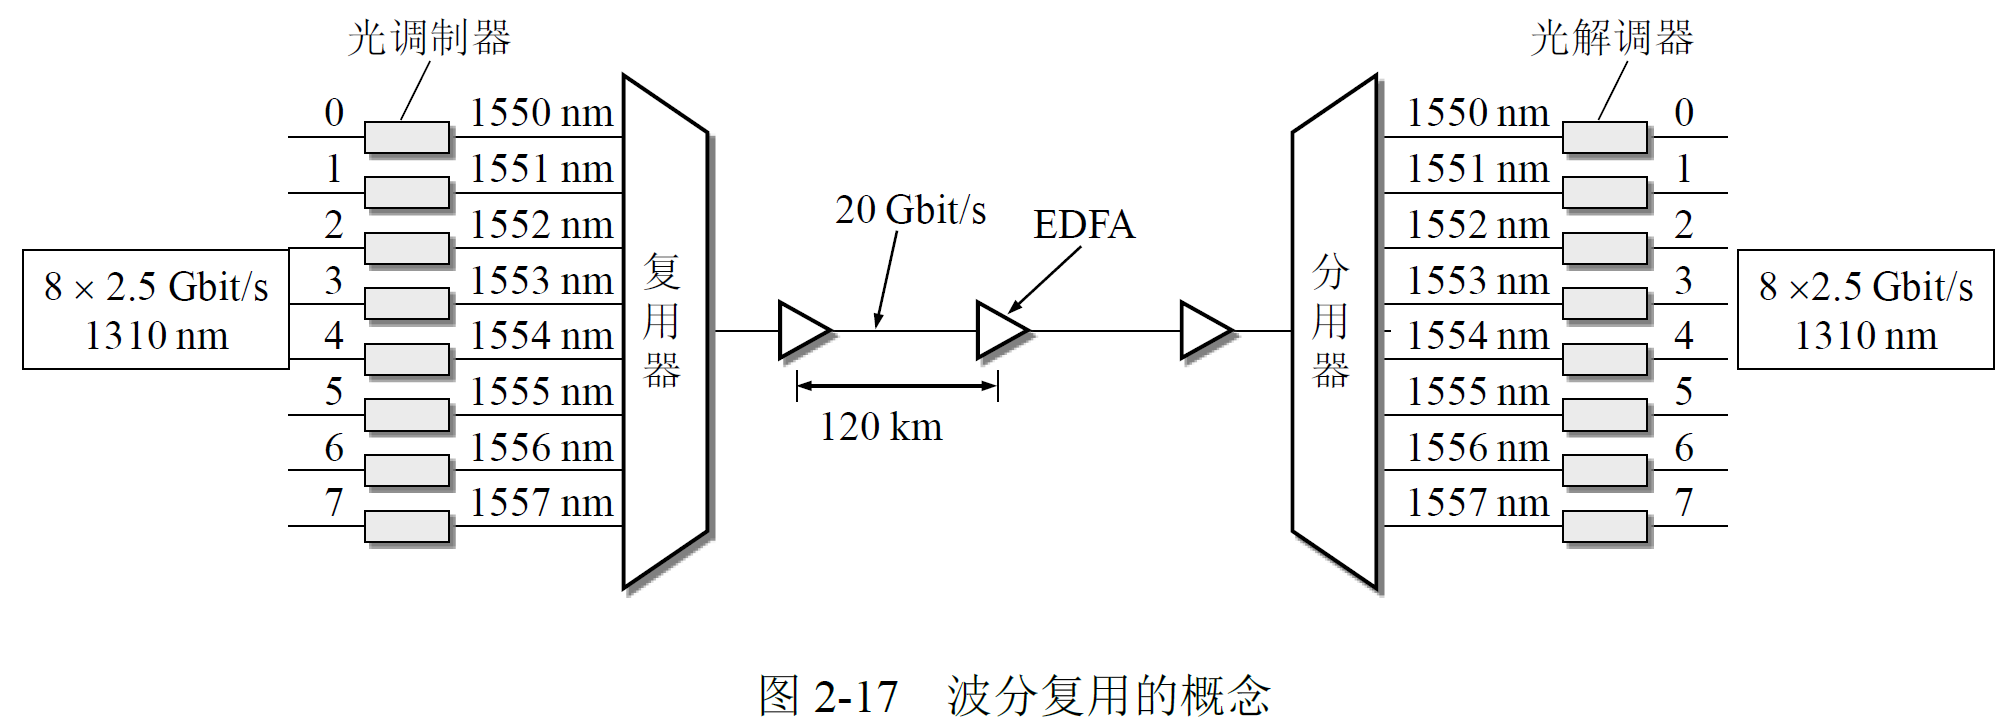
\includegraphics[width=0.9\textwidth]{img/2.17}
	\end{figure}

	\subsection{码分复用}

	\begin{itemize}
		\item 码分复用 CDM 是另一种共享信道的方法。实际上,由于该技术主要用于多址接入,人们更常用的名词是码分多址 CDMA
		\item CDM 的每一个用户可以在同样的时间使用同样的频带进行通信
		\item 由于各用户使用经过特殊挑选的不同码型,因此各用户之间不会造成干扰
		\item CDM 最初是用于军事通信的,因为这种系统所发送的信号有很强的抗干扰能力,其频谱类似于白噪声,不易被敌人发现
		\item 随着技术的进步,CDMA 设备的价格和体积都大幅下降,因而现在已广泛用于民用的移动通信中
	\end{itemize}

	\begin{figure}[H]
		\centering
		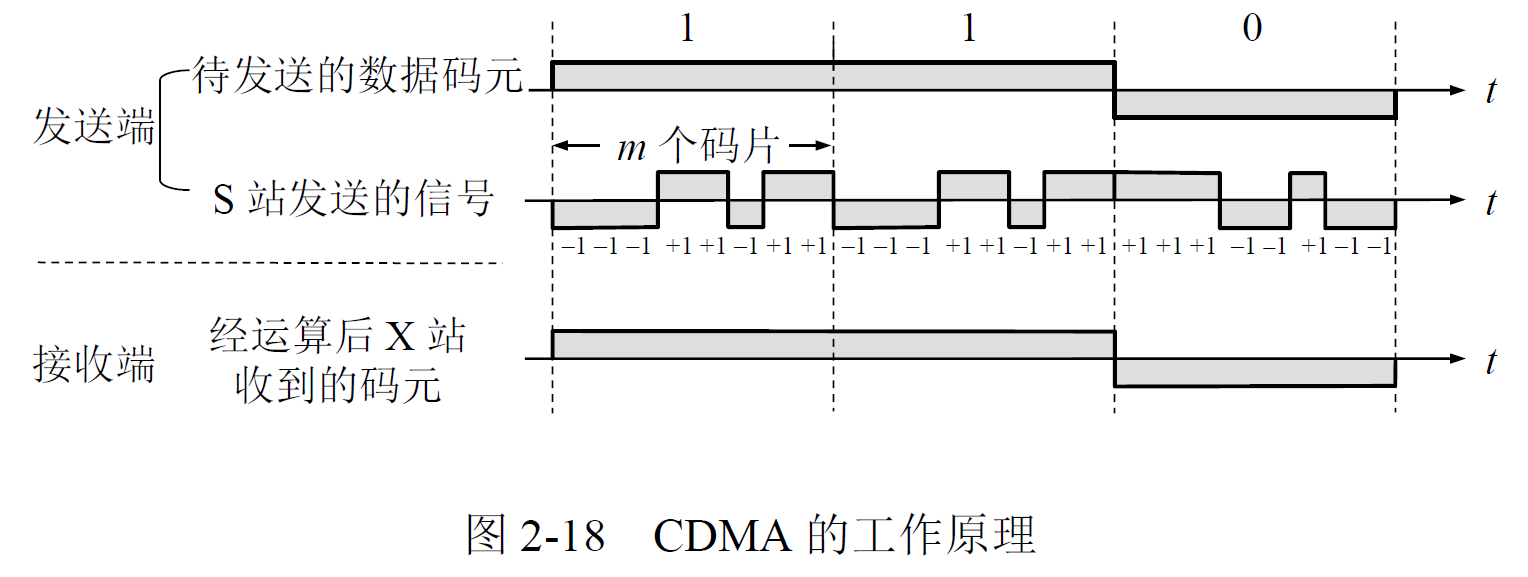
\includegraphics[width=0.75\textwidth]{img/2.18}
	\end{figure}

	\begin{itemize}
		\item 在CDMA中,每一个比特时间再划分为 $m$ 个短的间隔,称为码片(chip)。通常 $m$ 的值是64或128
		\item 使用 CDMA 的每一个站被指派一个唯一的 $m \ \mathrm{bit}$ 码片序列
		\begin{itemize}
			\item 一个站如果要发送比特1,则发送它自己的 $m \ \mathrm{bit}$ 码片序列
			\item 一个站如果要发送比特0,则发送它自己的 $m \ \mathrm{bit}$ 码片序列的二进制反码
		\end{itemize}
		\item 码片序列的挑选原则为:
		\begin{itemize}
			\item 分配给每个站的码片序列必须各不相同,实际常采用伪随机码序列
			\item 分配给每个站的码片序列必须互相正交,即规格化内积为0
		\end{itemize}
		\item 令向量 $\boldsymbol{S}$ 表示站 $S$ 的码片序列,向量 $\boldsymbol{T}$ 表示其他任何站的码片序列,则有:
		$$
		\begin{aligned}
			\boldsymbol{S}\cdot \boldsymbol{T} & =\frac{1}{m}\sum_{i=1}^m S_iT_i=0 \\
		\boldsymbol{S}\cdot \overline{\boldsymbol{T}}=0\quad\quad\quad\quad
		& \boldsymbol{S}\cdot \boldsymbol{S}=1\quad\quad\quad\quad
		\boldsymbol{S}\cdot \overline{\boldsymbol{S}}=-1
		\end{aligned}
		$$
	\end{itemize}

	\textbf{例:}站点 A、B、C 通过 CDMA 共享链路,A、B、C 的码片序列分别是$(1,1,1,1)$、$(1,-1,1,-1)$和$(1,1,-1,-1)$。若 C 从链路上收到的序列是$(2,0,2,0,0,-2,0,-2,0,2,0,2)$,则 C 收到 A 发送的数据是\ \underline{101} 

\end{document}


